% Drawing 81/03-1 -- folder 81, batch 03, archive page 54 (PDF page 55).
% Transcription: page sans texte : croquis au crayon d'une même opération de collage en volume — un disque vu en perspective relié par un tube court à une feuille rectangulaire ; un petit cercle traversé d'un trait entre deux arcs ; un grand rectangle à qui une bande est attachée par le haut ; une feuille en perspective portant deux petits cylindres dressés. En haut à droite, à l'encre, le trait vertical à extrémités recourbées du premier croquis de la page 53
% Kind: page of pencil sketches of a gluing in volume. Method 2 (schematic redraw from the facsimile). Status: ok.
% Notes: Faint pencil, redrawn at its places: a disk seen in perspective (two offset ellipses, the near rim heavy where he inked it) joined by a short tube (two lines, small rings at its ends) to a sheet standing behind it (its top edge and right edge) with a rectangular piece below the tube (heavy stroke at its upper left); a small circle crossed by a stroke between two arcs; a large rectangle with a band (two verticals and a U) attached at its top, its sides joined at the bottom to the sheet below; a sheet in perspective carrying two small upright cylinders, with the strokes of its edges as drawn; at the top right, in ink, the two small curled marks (from p. 53) and the faint stroke between them. Faint doublings reduced to one stroke. Still differs: the edges of the lower sheet are a reading of overlapping faint strokes. Redrawn 2026-11-09 (issue 128): to check again. 2026-11-14, Claude Opus 5.5, overlay check (issue 147): every sketch re-read on gridded crops of the 400 dpi colour scan (30 to 50 px per unit), rasterised from its own coordinates over it and measured (all pencil of the page within 1.5 units of a stroke, except three specks and a stain; the faint pencil arcs within about 1 unit of their strokes); not compiled (no TeX in the session). Changed: the second ellipse of the disk is not a closed ellipse on the page: it is drawn as the arcs that are there (its left side inside the outline, its upper right arc, and a fainter outer arc beyond it, broken where the tube crosses it), with the short stroke that closes the disk at the lower right; the near rim, heavy, ends in a short heavy stroke into the tube, which is crossed by a thin oblique stroke; the tube is doubled below; the ring at its near end moved onto its ink; its far end is a rounded loop of two strokes (not a flat ring), with the two heavy strokes beyond it; the piece below the tube is drawn as one stroke along its left side, rounded bottom and right side, with the strokes that cross under its lower left corner and the faint doubling of its right side, and the heavy hooked stroke at its upper left; the left edge of the sheet behind is two strokes running down into the piece. The small circle crossed by a stroke and its two arcs, the rectangle (its corners and the kink of its right side as drawn), the band, the lower sheet with its edges, and the two cylinders (each redrawn as its strokes: the left one a short one beside a taller narrow one, the right one with its heavy curl at the foot, the line from its top rising to the right and the strokes through its foot) lie on their pencil. Left out: three specks of ink and a stain at the upper left of the sheet. Status set to ok.
% Coordinates: 1 unit = 1 mm = 1/100 of the crop width (bbox in page fractions: [0.08, 0.06, 0.97, 0.7]).
% Redrawn by Claude (claude-opus-5-5), issue #73, 2026-11-09; not checked by a human; not compiled (no TeX in the session).
% Checked by Claude (claude-opus-5-5) 2026-11-14 (issue #147): overlaid on the 400 dpi colour facsimile, corrected; not compiled (no TeX in the session). Not checked by a human. Status: ok.
% Rights: reproduces part of the work -- behind RENDER_TRANSCRIPTS, never published by itself.
\documentclass[tikz,border=3pt]{standalone}
\usepackage{amsmath,amssymb}
\usetikzlibrary{patterns,arrows.meta}
\tikzset{pencil/.style={black!45}, struck/.style={black!35}, mark/.style={circle,draw,inner sep=1.3pt}, pt/.style={circle,fill,inner sep=0.9pt}, opt/.style={circle,draw,fill=white,inner sep=1.1pt}}
\begin{document}
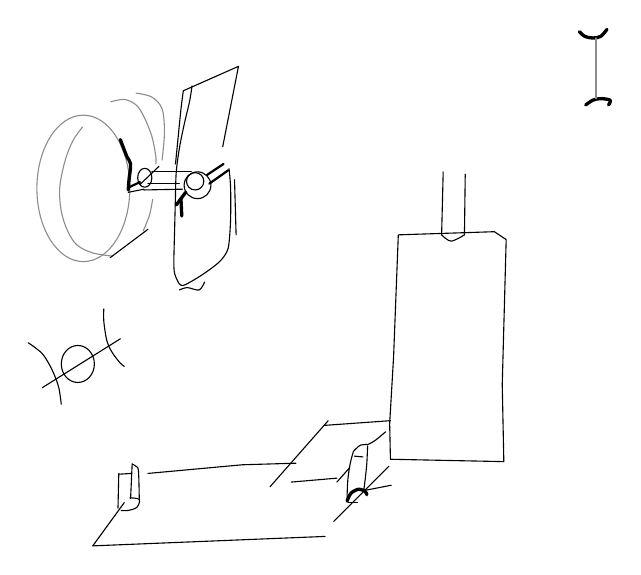
\begin{tikzpicture}[x=1mm,y=1mm,line cap=round,line join=round,font=\scriptsize]
\draw[pencil] (19.8,-30.1) ellipse[x radius=5.9, y radius=9.3];
\draw[pencil] plot[smooth, tension=0.55] coordinates {(19.7,-22.3) (18.5,-24) (17.5,-26.5) (16.8,-30) (17,-33) (17.8,-35.5) (19,-37.3) (21,-38.3) (23.5,-38.7)};
\draw[pencil] plot[smooth, tension=0.55] coordinates {(23.3,-19.1) (25,-18.8) (26.5,-19.5) (27.5,-21) (28.5,-23.5) (29,-26) (29,-27)};
\draw[pencil] plot[smooth, tension=0.55] coordinates {(26.5,-18) (28.5,-18.5) (29.8,-20) (30.1,-23) (29.8,-26.5)};
\draw[pencil] plot[smooth, tension=0.55] coordinates {(28.6,-31.5) (28.2,-33.5) (27.4,-35.5)};
\draw (23.2,-38.9) -- (28,-35.3);
\draw[very thick] plot[smooth, tension=0.55] coordinates {(24.5,-23.9) (25.3,-26) (25.8,-27) (25.6,-29) (25.5,-30.3)};
\draw[thick] (25.5,-30) -- (27,-29.3);
\draw (27,-29.6) -- (29.4,-27.3);
\draw (25.5,-30.6) -- (27.5,-30.2);
\draw (27.6,-28.75) ellipse[x radius=0.9, y radius=1.2];
\draw (28.5,-28) -- (33.5,-28);
\draw (27.5,-30.3) -- (32.4,-30.2);
\draw (28,-29.5) -- (32,-29.5);
\draw (34.3,-29.7) ellipse[x radius=1.7, y radius=1.7];
\draw (34,-29.2) ellipse[x radius=1.1, y radius=1.1];
\draw[thick] (35.5,-28.4) -- (37.6,-27);
\draw[thick] (35.8,-29.5) -- (38.2,-27.8);
\draw (32.5,-17.7) -- (39.5,-14.6) -- (37.5,-24.8);
\draw plot[smooth, tension=0.55] coordinates {(33.6,-17.1) (33.3,-19) (32.6,-22) (32,-25) (31.6,-28) (31.5,-31)};
\draw plot[smooth, tension=0.55] coordinates {(32.5,-17.7) (32.2,-20) (31.8,-24) (31.5,-27)};
\draw plot[smooth, tension=0.55] coordinates {(31.5,-31) (31.4,-35) (31.3,-40) (31.6,-41.5) (32.2,-42.4) (33,-42.2) (35,-41) (37,-39.5) (38,-38.2) (38.3,-37) (38.5,-34) (38.5,-30) (38.3,-27.6)};
\draw plot[smooth, tension=0.55] coordinates {(32,-43) (33,-42.7) (34.5,-43) (35.2,-42)};
\draw (39,-29) -- (39.2,-36);
\draw[very thick] (32.2,-31.5) -- (32.3,-33.6);
\draw[very thick] (32.8,-30.6) -- (31.6,-32.2);
\draw (19.1,-52.4) ellipse[x radius=2.1, y radius=2.35];
\draw (14.6,-55.4) -- (24.5,-49.2);
\draw plot[smooth, tension=0.55] coordinates {(12.8,-49.7) (14.5,-51) (15.5,-52.5) (16.2,-54) (16.7,-55.5) (17,-57.5)};
\draw plot[smooth, tension=0.55] coordinates {(22.4,-45.4) (22.4,-47) (22.8,-49.5) (23.5,-51) (24.5,-52.3) (25,-52.7)};
\draw (59.8,-36) -- (72,-35.6) -- (73.5,-36.6) -- (73,-55) -- (73.2,-64.8) -- (58.8,-64.5) -- (58.7,-60) -- (59.2,-51.5) -- cycle;
\draw (65.5,-28) -- (65.3,-36);
\draw (68.3,-28.3) -- (68.2,-36);
\draw plot[smooth, tension=0.55] coordinates {(65.3,-36) (66.5,-36.8) (68.2,-36)};
\draw (50.4,-60.2) -- (58.8,-59.6);
\draw (50.9,-59.6) -- (43.5,-68);
\draw (21,-75.5) -- (50.5,-74.3);
\draw (28,-66.3) -- (40,-65.2) -- (46.8,-65);
\draw (25,-70) -- (21,-75.5);
\draw (46.2,-67.4) -- (52,-66.9);
\draw (52,-67.4) -- (53.6,-65.6);
\draw (51.6,-72.4) -- (58.6,-65.4);
\draw (55.3,-68.5) -- (58.9,-67.8);
\draw plot[smooth, tension=0.55] coordinates {(54.1,-63.5) (55,-62.7) (56,-62.6) (57,-62) (58.2,-61)};
\draw (54.2,-64.1) -- (55.3,-64.2);
\draw plot[smooth, tension=0.55] coordinates {(54.1,-63.5) (53.7,-65) (53.4,-67) (53.3,-69) (53.3,-69.8)};
\draw plot[smooth, tension=0.55] coordinates {(55.9,-62.8) (55.8,-65) (55.6,-67) (55.4,-68.5)};
\draw[very thick] plot[smooth, tension=0.55] coordinates {(53.3,-69.8) (53.8,-68.8) (54.8,-68.3) (55.6,-68.6) (55.8,-69)};
\draw (53.4,-70) -- (54.6,-70);
\draw (24.3,-66.3) -- (24.2,-70.7);
\draw (24.3,-66.4) -- (25.9,-66.3);
\draw (26,-65.1) -- (25.8,-69.5);
\draw plot[smooth, tension=0.55] coordinates {(26,-65.1) (26.5,-65.4) (26.8,-66) (26.9,-69.5)};
\draw plot[smooth, tension=0.55] coordinates {(25.7,-69.4) (26.9,-69.6) (26.6,-70.6) (25.5,-71) (24.6,-71)};
\draw[very thick] plot[smooth, tension=0.55] coordinates {(82.8,-10.2) (83.5,-10.8) (84.5,-11) (85.5,-10.8) (86.3,-9.9)};
\draw[very thick] plot[smooth, tension=0.55] coordinates {(83.6,-19.5) (84.5,-18.9) (85.5,-18.7) (86.7,-18.9) (86.5,-19.5)};
\draw[pencil] (84.9,-11) -- (84.9,-18.7);
\end{tikzpicture}
\end{document}
